\documentclass{amsart}
\usepackage{amssymb}
\usepackage{graphics}
\usepackage{graphicx}
\usepackage{verbatim}
\usepackage{amssymb, epsfig}
\usepackage[leqno]{amsmath}
\usepackage{eurosym}
\usepackage{listings}

\def\P{\mathbb{P}}
\def\Q{\mathbb{Q}}
\def\E{\mathbb{E}}

\newtheorem{theorem}{Theorem}[section]
\newtheorem{lemma}[theorem]{Lemma}
\newtheorem{proposition}[theorem]{Proposition}
\newtheorem{example}[theorem]{Example}
\newtheorem{definition}[theorem]{Definition}
\newtheorem{corollary}[theorem]{Corollary}
\newtheorem{remark}[theorem]{Remark}
\newtheorem{assumption}[theorem]{Assumption}

\textheight=9.5 in
\textwidth=6.5in
\topmargin=-.0in
\hoffset=-.75in

\title{Monte Carlo Option Pricing Dashboard}
\author{Steve Taylor: staylor@continuum.io}
%\author{Eric Hendries, Jun Huang, Ruixue Li, Xiao Li, Yiyang Qi, Helene Sajer, Stephen Taylor, John 
%Zerolis}
%\email{Corresponding Author: Stephen Taylor, Morgan Stanley, Email: steve98654-at-gmail.com}

\begin{document}

\maketitle
\begin{abstract}
    This document outlines the motivation for the Monte Carlo simulation based option pricing 
    dashboard as well as a brief technical description of its backend methods.
    It also describes all the inputs and outputs of the dashboard and provides several screen shots
    that demonstrate usage. 
\end{abstract}

\section{Motivation for Dashboard and Technical Description of Methods}

Ito processes are widely used to simulate financial quantities including stock prices, interest rates, 
yield spreads, etc.  In particular, on common application involves simulating multiple paths of 
a single stock's price and using the results to value European options. This involves specifying the initial value $X_0>0$ of the stock that one would like to simulate, defining the drift function, $\mu(x)$, and setting volatility function $\sigma(x)>0$ of a one dimensional Ito process:
%
\begin{equation}
    dX_t = \mu(X_t)dt + \sigma(X_t)dW_t \label{ito}
\end{equation}
% 
where here we let $X_t$ denote the process itself, $dt$ the infinitesimal time step, and 
$W_t$ a Brownian motion.  For example, in the Black Scholes lognormal model, the drift function is taken to be
$\mu(x)=rx$ and the volatility function is $\sigma(x)=\sigma x$ where $r$ is the constant risk-free 
rate and $\sigma$ is a constant log-normal volatility. 

In order to initialize a Monte Carlo simulation of this process, one needs to specify the number of paths $m$ that will be generated as well as the number of points $n$ that each path 
will contain.  Next, one needs to specify the timestep $\Delta t>0$ between time points in 
the simulation (we will take a uniformly spaced time grid); the time elapsed at the $i$-th step of the 
simulation is then $T_i=i\Delta t$.    

Now that the parameters of the simulation are defined, we must select a discretization 
scheme for equation (\ref{ito}).  There are a variety of ways to carry our this process and 
we will consider three such schemes: the Euler, Milstein, and a Predictor/Corrector (Pred/Corr) method. 

Each scheme iteratively builds up simulated paths whose values we represent by $X_i^j$ where here 
$i$ denotes the time step and $j$ the path number. We let $\mathcal{N}(0,\sigma^2)$ denote 
a draw from a normal random variable with mean zero and variance $\sigma^2$.  
The Euler scheme for a single path is then generated by: 
%
\begin{equation}
    X_{i+1}^j = X^j_i + \mu(X_i^j)\Delta t + \sigma(X_i^j)\mathcal{N}(0,\Delta t).
\end{equation}
%
The Milstein Scheme provides a second order correction to the Euler scheme, has smaller 
discretization error, and is given by 
\begin{equation}
    X_{i+1}^j = X_i^j + \mu(X_i^j)\Delta t + \sigma(X_i^j)\mathcal{N}(0,\Delta t)
    +\frac{1}{2}\sigma(X_i^j)\sigma'(X_i^j)\left( \mathcal{N}(0,\Delta t )^2 -\Delta t\right).
\end{equation}

We also consider a Predictor Corrector Method \cite{Klo} that generally has better stability properties 
over the Milstein Scheme \cite{Klo} and is specified by:  
\begin{equation}
    \tilde{X}_{i+1}^j = X_i^j + \mu(X_i^j)\Delta t + \sigma(X_i^j)\mathcal{N}(0,\Delta t)
\end{equation}
%
\begin{equation}
    X_{i+1}^j = X_i^j + \frac{1}{2} (\bar{\mu}(\tilde{X}_{i+1}^j)+\bar{\mu}(\tilde{X}_{i+1}^j)) \Delta t
    + \frac{1}{2}(\bar{\mu}(\tilde{X}_{i+1}^j)+\bar{\sigma}(\tilde{X}_{i+1}^j))\mathcal{N}(0,\Delta t)
\end{equation}
%
where here $\bar{\mu(x)}\equiv \mu(x) - \frac{1}{2}\sigma(x)\sigma'(x)$. 

After the paths $X_i^j$ have been simulated, if at time $T_i$ we would like to price an 
option with strike $K$ that has payoff function, $\max(X-K,0)$, then we can use our Monte Carlo 
results at the $i$-th time step to compute the mean and variance of the simulated option prices 
%
\begin{equation}
    \mathbb{E}(\max(X-K,0)) \approx \frac{1}{m}\sum_{j=1}^m \max(X_i^j - K,0)\equiv\hat{\mu}_K
\end{equation}
\begin{equation}
    \mathrm{Var}(\max(X-K,0)) \approx \frac{1}{m}\sum_{j=1}^m \max(X_i^j - K,0)^2 - \hat{\mu}_K^2
    \equiv \hat{\sigma}^2_K
\end{equation}
%
Then assuming that the number of paths is large enough, the central limit theorem implies that 
the Monte Carlo estimate $\hat{\mu}_K$ is the price of the option, which has a one-sigma 
error bound of $[\hat{\mu}_K-\hat{\sigma}_K/\sqrt{m}, \hat{\mu}_K+\hat{\sigma}\sqrt{m}]$.

We now describe how this information is incorporated into our dashboard.

\section{Description of Inputs and Outputs}

We first list, describe the meaning of, and provide examples for all the inputs in our dashboard. 

\begin{enumerate}
    \item Drift Function: the drift function $\mu(x)$ in equation (\ref{ito}), e.g. $r*x$   
    \item Drift Derivative: the derivative of the drift function $\mu'(x)$ in equation (\ref{ito}), e.g. $r$  
    \item Volatility Function: the volatility function $\sigma(x)$ in equation (\ref{ito}), e.g. $\sigma*x$
    \item Volatility Derivative: the derivative of the volatility function $\sigma'(x)$ in equation (\ref{ito}), e.g $\sigma$. 
    \item Number of Paths: the number of paths in the Monte Carlo simulation, e.g. 500. 
    \item Number of Points: the number of points per path in the Monte Carlo simulation, e.g. 100 
    \item Histogram Line: the time step where to perform the Monte Carlo option pricing and
          density estimation, e.g. 50 if there are 100 total points per path 
    \item Initial Value: the starting value of the asset underlying the option that is to be priced, e.g. 10
    \item MC Scheme: the type of Monte Carlo scheme to run, e.g. Euler 
    \item Run Text Fields: Text field to run the Monte Carlo simulation after all other inputs have 
          been entered, e.g. type run, run1, etc. to start the simulation
\end{enumerate}

We now describe how the output statistics are computed and how the three plots in the 
dashboard are generated. 

\begin{enumerate} 
    \item Simulated Path Plot (top right):  In the background of this plot, we plot up to fifty simulated paths for the process set up in the inputs.  We also plot the mean path in the solid red line as well as one, two, and three sigma neighborhoods around the mean path.  A vertical line is also plotted in black which indicates the time step where the Monte Carlo simulation is being performed and the density of the path values at the time is being estimated below.
    \item Density Estimate Plot (bottom left): In the lower left plot title, we indicate the time that corresponds to the vertical black line in the top right plot where the Monte Carlo simulation is being performed as well as the mean and standard deviation of the points of the simulated paths at this time.  In the plot, we use a nonparametric kernel density estimator using a Gaussian kernel and Scott's rule of thumb for bandwidth selection.  
    \item Option Price and Error Bar Plot (bottom right):  In the lower right plot, we compute the 
        price of a set of options with varying strike prices using the values of the simulated 
        paths that are plotted in the upper right plot at the time denoted by the vertical black line.  
        These prices are plotted in blue in the lower right plot.  We also compute the variance of these 
        prices and display one-sigma and two-sigma error bars for each price in red and green in this 
        figure. 
\end{enumerate} 

\section{Screenshots of Examples} 

We provide three examples of a mean reverting Ornstein-Uhlenbeck process, a normal Gaussian process, 
and a lognormal process below.  Feel free to copy the inputs to see how the dashboard works.

\begin{figure}[h!]
    \centering
    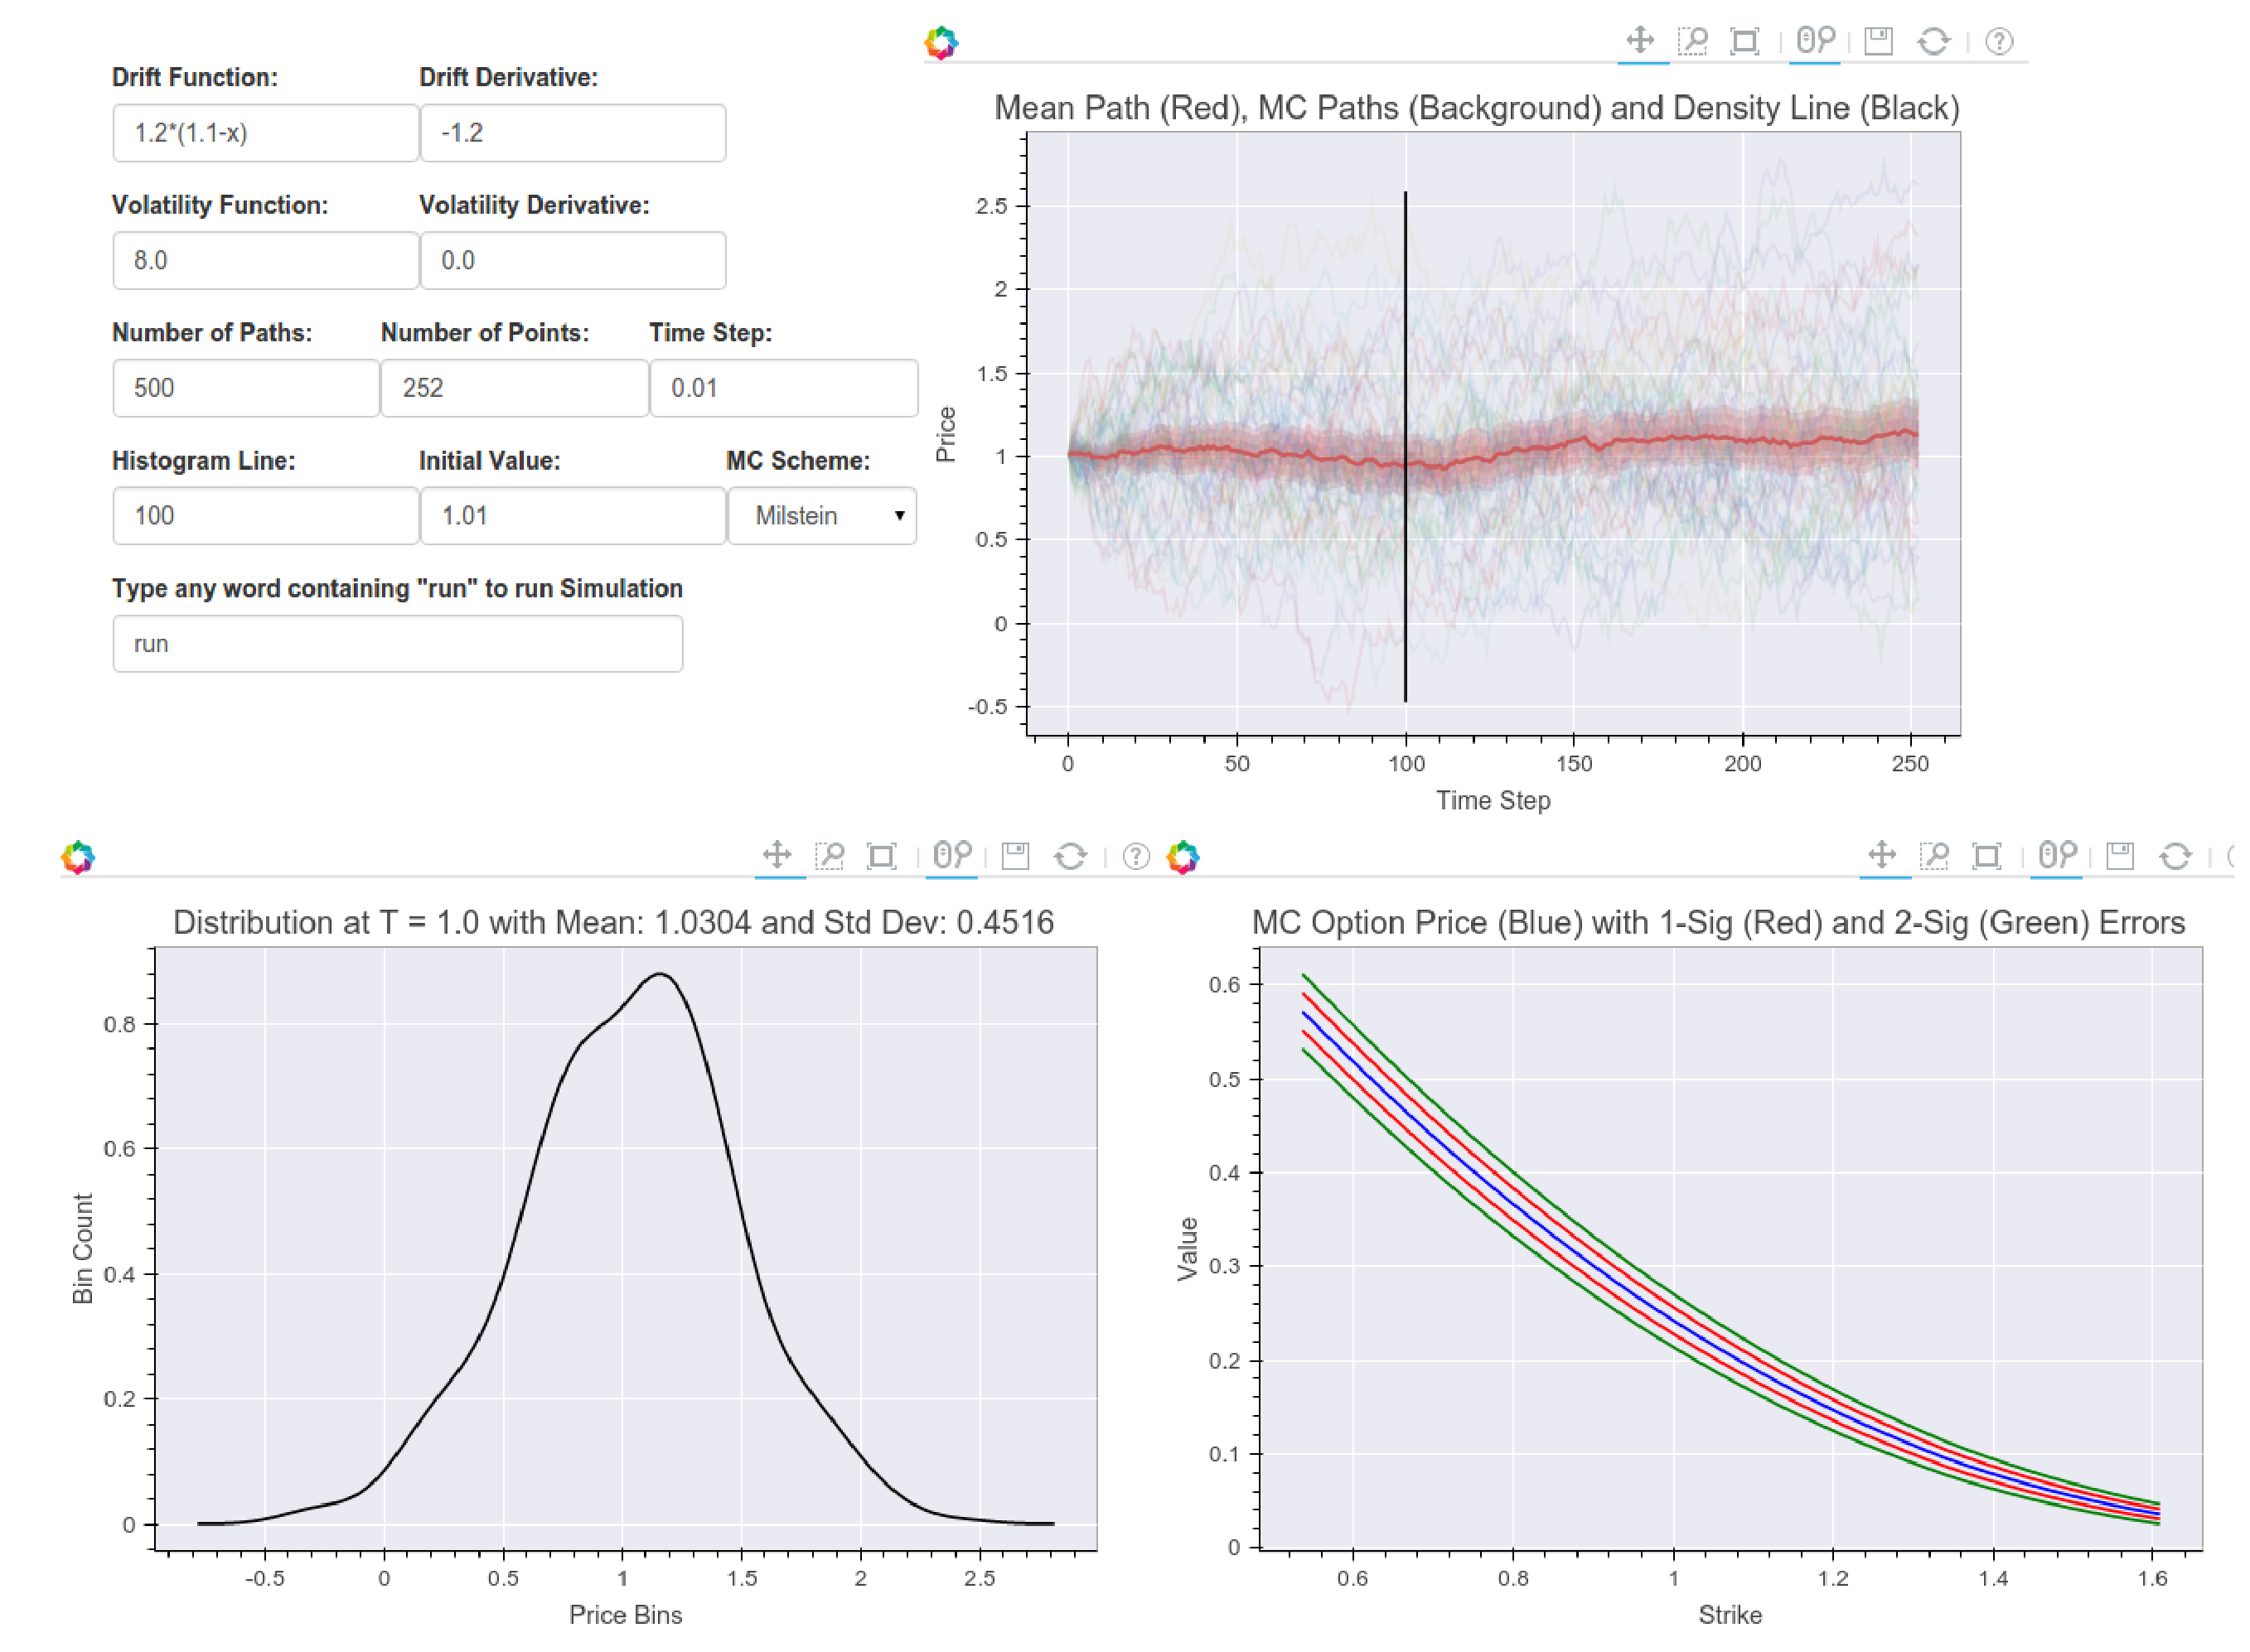
\includegraphics[width=0.8\textwidth]{fig1.eps}
    \caption{Orenstein-Uhlenbeck Example}
    \label{fig1}
\end{figure}


\begin{figure}[h!]
    \centering
    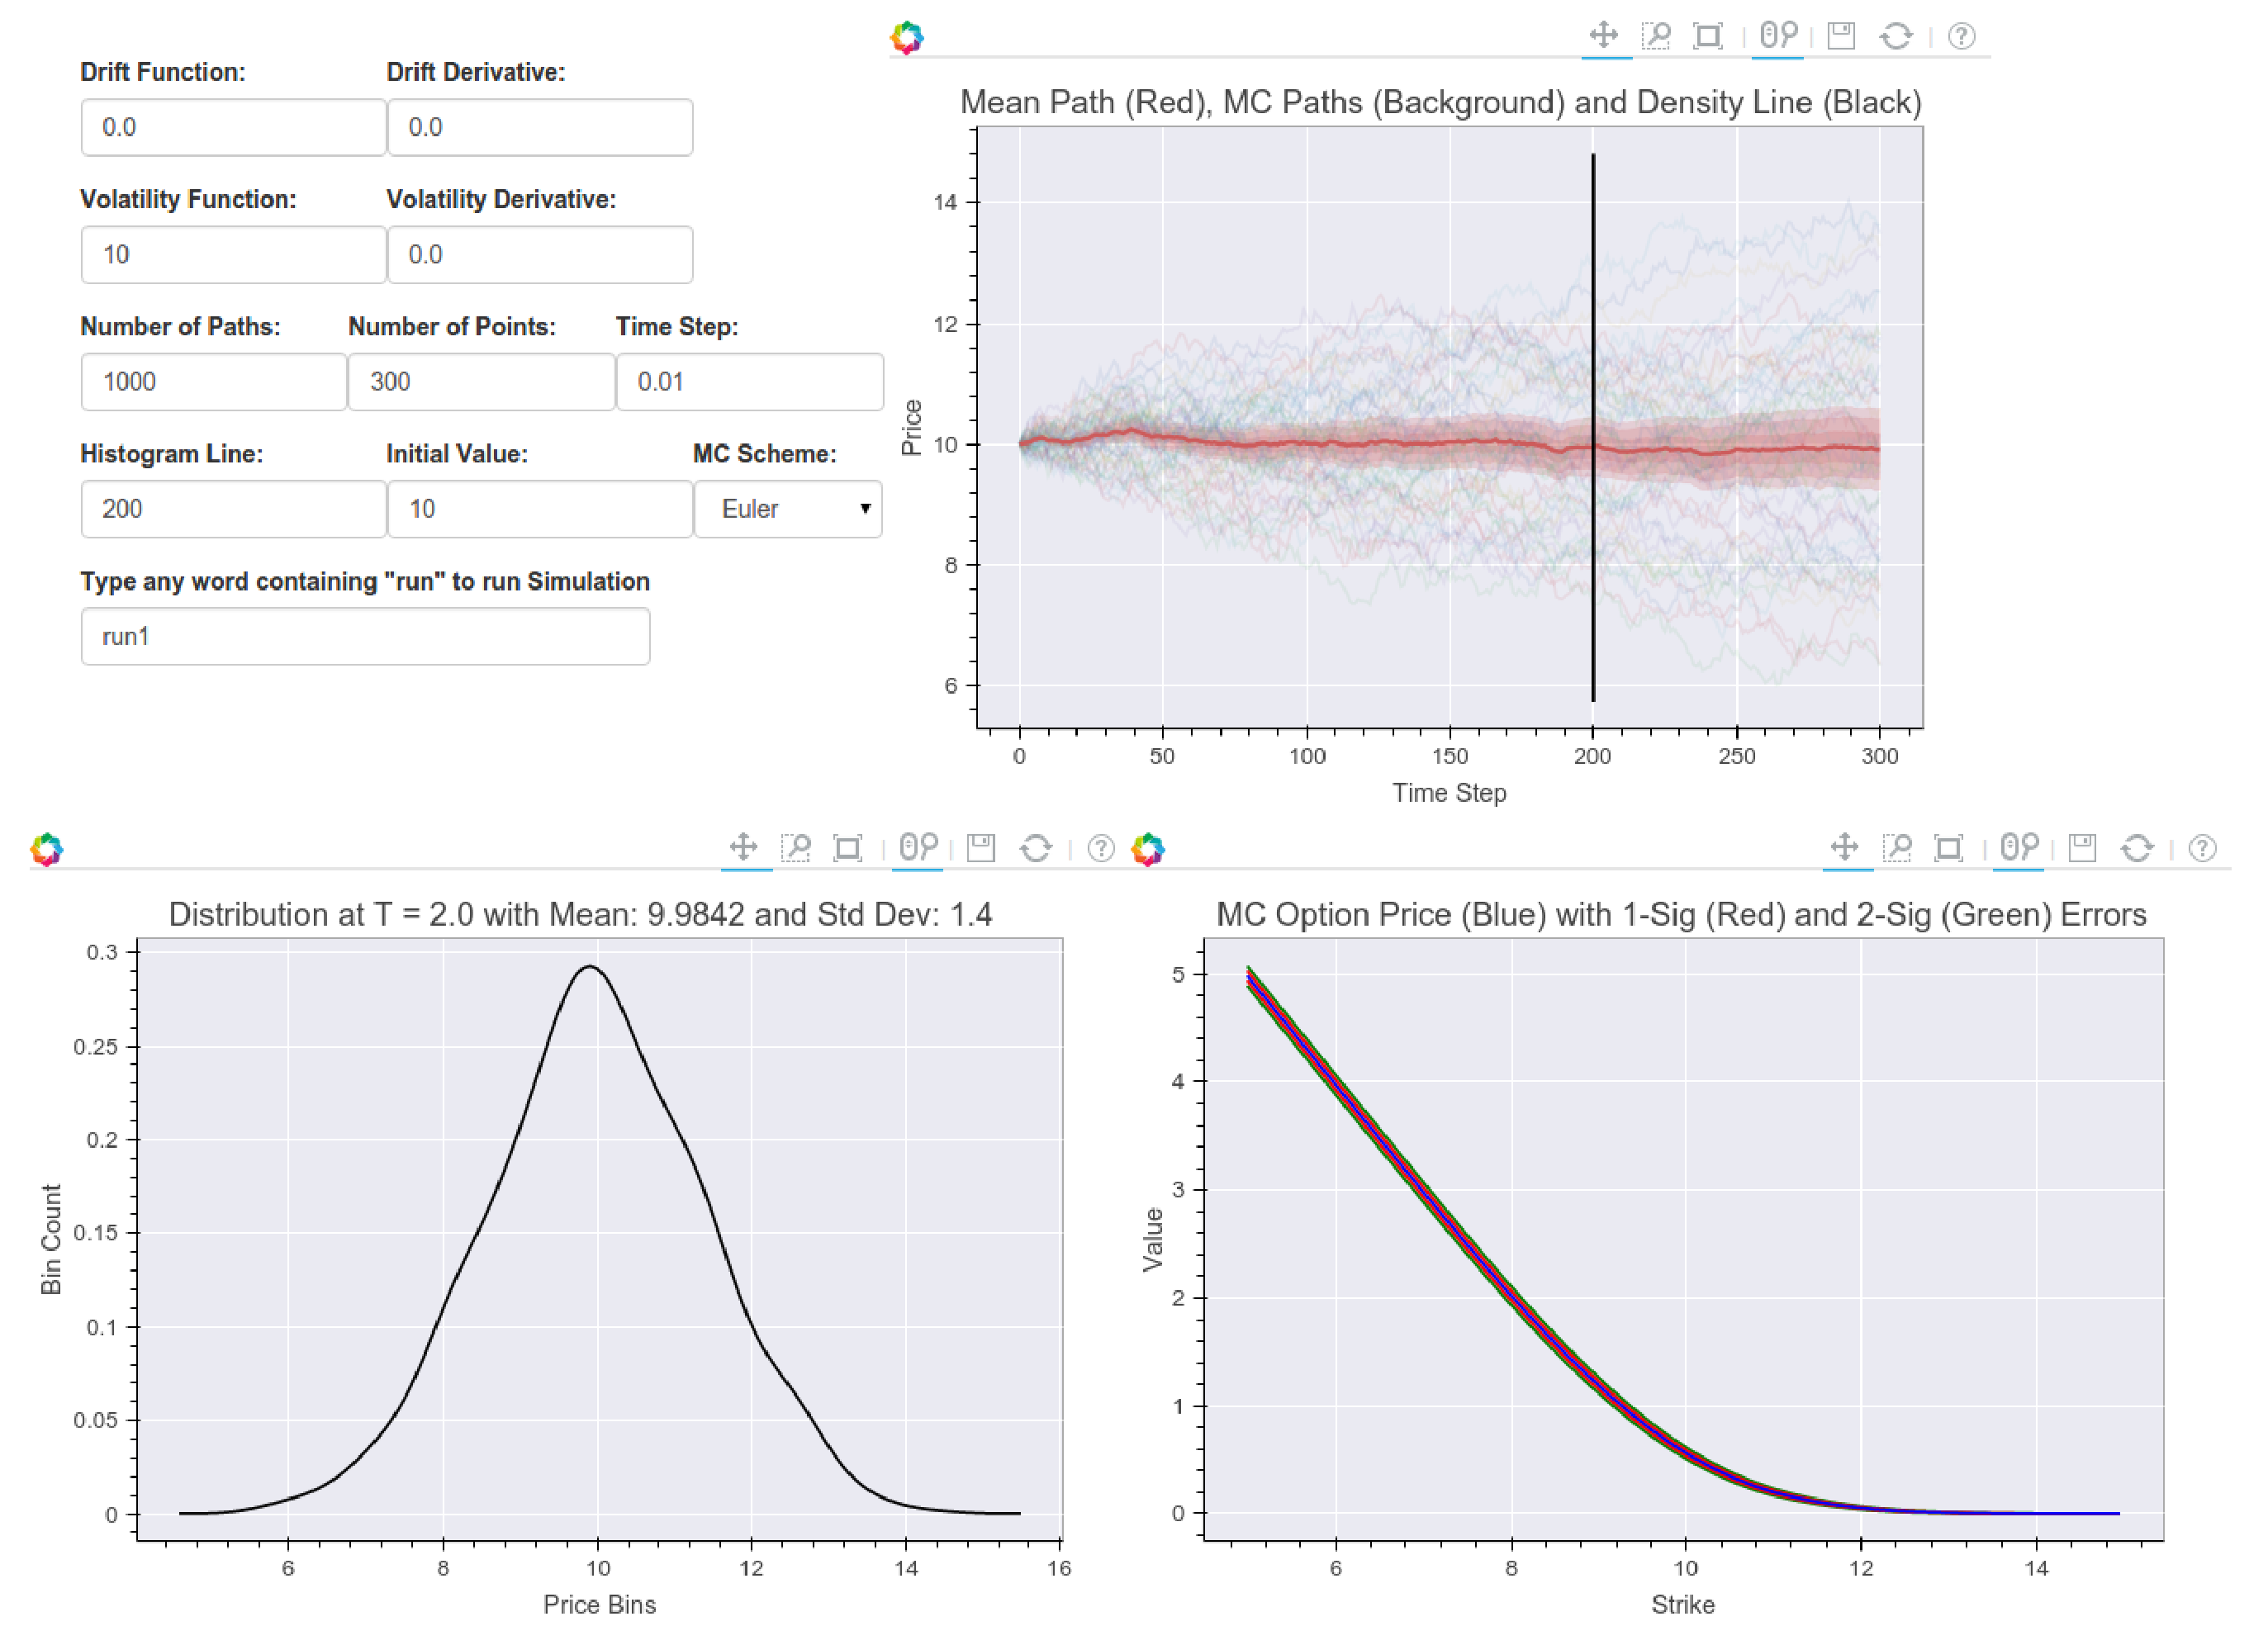
\includegraphics[width=0.8\textwidth]{fig2.eps}
    \caption{Normal Example}
    \label{fig2}
\end{figure}

\begin{figure}[h!]
    \centering
    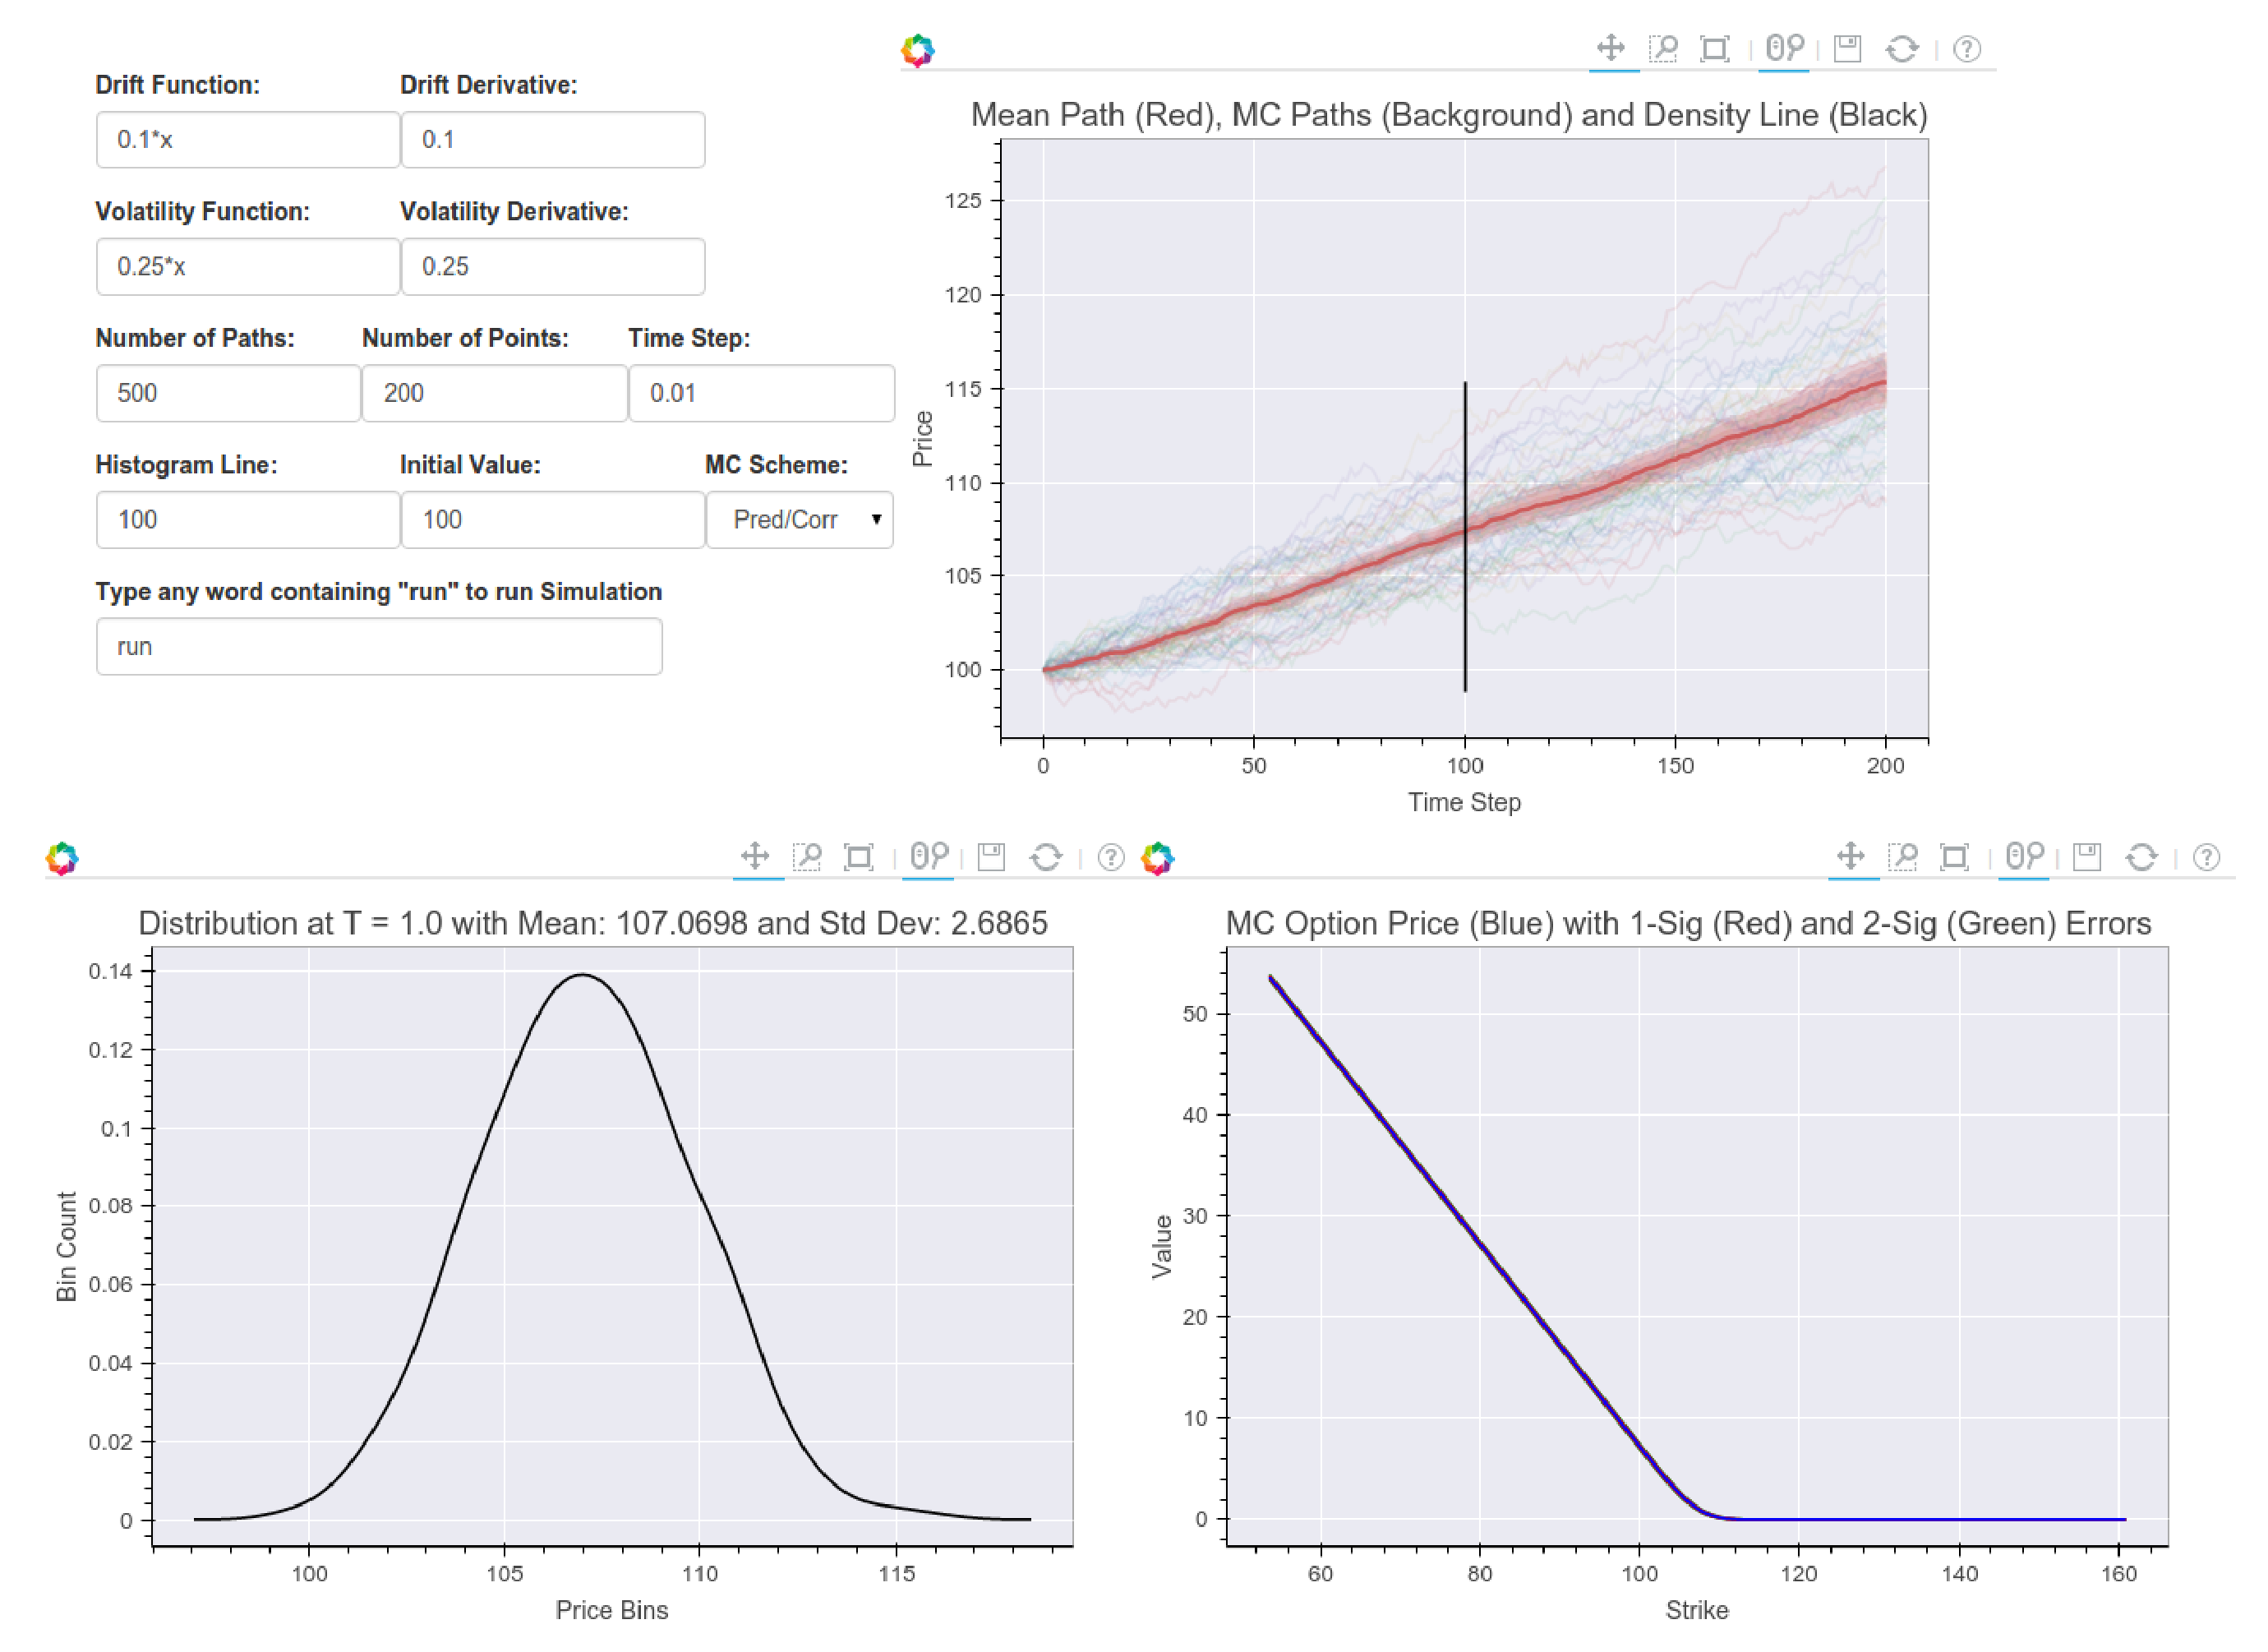
\includegraphics[width=0.8\textwidth]{fig3.eps}
    \caption{Lognormal Example}
    \label{fig3}
\end{figure}

\begin{thebibliography}{100}
\bibitem{Klo} http://www.qfrc.uts.edu.au/research/research\_papers/rp222.pdf
\end{thebibliography}
\end{document}

